\documentclass{standalone}
% \documentclass{article}

\usepackage{tikz}

\begin{document}

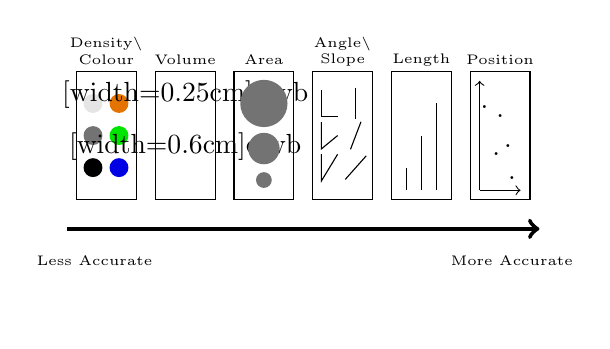
\begin{tikzpicture}
\draw[ultra thick, ->] (0, -0.25) -- (6, -0.25);
\node at (0, -1.3) {}; % In order to get gap at bottom

\def \m {0.12}

\draw (0+\m, \m) rectangle (1-\m, 1.75);
\draw (1+\m, \m) rectangle (2-\m, 1.75);
\draw (2+\m, \m) rectangle (3-\m, 1.75);
\draw (3+\m, \m) rectangle (4-\m, 1.75);
\draw (4+\m, \m) rectangle (5-\m, 1.75);
\draw (5+\m, \m) rectangle (6-\m, 1.75);

\node at (0.35, -0.65) {\tiny{Less Accurate}};
\node at (5.65, -0.65) {\tiny{More Accurate}};

% Density/Colour
\node at (0.5, 2.1) {\tiny{Density\textbackslash}};
\node at (0.5, 1.9) {\tiny{Colour}};
\draw[draw=none, fill=black] (0.33, 0.4075+\m) circle (0.12);
\draw[draw=none, fill=black!55] (0.33, 0.815+\m) circle (0.12);
\draw[draw=none, fill=black!10] (0.33, 1.2225+\m) circle (0.12);
\draw[draw=none, fill=blue!90!black] (0.66, 0.4075+\m) circle (0.12);
\draw[draw=none, fill=green!90!black] (0.66, 0.815+\m) circle (0.12);
\draw[draw=none, fill=orange!90!black] (0.66, 1.2225+\m) circle (0.12);


% Volume
\node at (1.5, 1.9) {\tiny{Volume}};
\node at (1.5, 1.45) {\includestandalone[width=0.25cm]{ciwb}};
\node at (1.5, 0.8) {\includestandalone[width=0.6cm]{ciwb}};

% Area
\node at (2.5, 1.9) {\tiny{Area}};
\draw[draw=none, fill=black!55] (2.5, 0.25+\m) circle (0.1);
\draw[draw=none, fill=black!55] (2.5, 0.65+\m) circle (0.2);
\draw[draw=none, fill=black!55] (2.5, 1.2225+\m) circle (0.3);

% Angle/Slope
\node at (3.5, 2.1) {\tiny{Angle\textbackslash}};
\node at (3.5, 1.9) {\tiny{Slope}};
\draw (3.6666, 1.2225+\m+0.2) -- (3.6666, 1.2225+\m-0.2);
\draw (3.7333, 0.815+\m+0.175) -- (3.6, 0.815+\m-0.175);
\draw (3.8, 0.4075+\m+0.15) -- (3.5333, 0.4075+\m-0.15);
\draw (3.23, 1.2225+\m+0.17) -- (3.23, 1.2225+\m-0.17) -- (3.4366, 1.2225+\m-0.17);
\draw (3.23, 0.815+\m+0.17) -- (3.23, 0.815+\m-0.17) -- (3.4366, 0.815+\m);
\draw (3.23, 0.4075+\m+0.17) -- (3.23, 0.4075+\m-0.17) -- (3.4366, 0.4075+\m+0.17);

% Length
\node at (4.5, 1.9) {\tiny{Length}};
\draw (4+\m+0.19, 2*\m) -- (4+\m+0.19, 0.4075+\m);
\draw (4+\m+0.38, 2*\m) -- (4+\m+0.38, 0.815+\m);
\draw (4+\m+0.57, 2*\m) -- (4+\m+0.57, 1.2225+\m);

% Position
\node at (5.5, 1.9) {\tiny{Position}};
\draw[->] (5+2*\m, 2*\m) -- (6-2*\m, 2*\m);
\draw[->] (5+2*\m, 2*\m) -- (5+2*\m, 1.75-\m);
\foreach \Point in {(5.3, 1.3), (5.5, 1.18), (5.6, 0.8), (5.45, 0.7), (5.65, 0.4)}{
    \node at \Point {.};
}


\end{tikzpicture}

\end{document}
